\section{Cell-Donor Matching: Procedure, Assumptions and Limits}
\label{app:matching}

Figure~\ref{fig:cell-donor} illustrates the procedure, Algorithm~\ref{alg:match} specifies the
steps, and Table~\ref{tab:notation} defines the notation.

\subsection*{E.1 The procedure}

Both surveys are partitioned by the same two variables, per-capita income quintile $q$ and
province $p$, into $|\mathcal{C}| = 45$ cells $c = (q, p)$. For each \ac{NIDS} record $i$ with
cell $c(i)$, one donor $d$ is drawn from the \ac{FinScope} records in the same cell with
probability $w_d / \sum_{d' \in c(i)} w_{d'}$, where $w$ is the \ac{FinScope} household weight,
and the donor's six-flag vector (banked; store card; revolving credit; hire purchase; short-term
loan; personal loan) is copied to $i$ in its entirety. Draws are with replacement, seeded (42), and
the quintile of a \ac{FinScope} donor is assigned from the midpoint of its seven-band income
question divided by household size, against the weighted \ac{NIDS} quintile bounds. The
procedure is specified to fall back to the quintile-only pool if a cell is empty; no draw ever did.

The smallest cell holds 30 donors and the median 87; only three cells (all in the top
quintile: Limpopo, North West, Northern Cape) hold fewer than 50. Of 4{,}969 available donors,
3{,}597 were used at least once; the median donor was used twice, the 99th percentile 13 times,
and the most-used donor 20 times. Donor reuse is concentrated where \ac{NIDS} is dense and
\ac{FinScope} is thin: in the largest cell, the bottom quintile of KwaZulu-Natal, 1{,}058
recipients drew from 109 donors, and eleven cells have more than three recipients per donor.
The heaviest 1\% of donors nonetheless supply only 5.1\% of recipients.

\subsection*{E.2 Assumptions under which the match is credible}

\begin{description}
\item[A1. Cell sufficiency.] Conditional on income quintile and province, the six flags are
independent of everything else in \ac{NIDS} that affects a household's behaviour in the model.
This assumption cannot be tested from the two surveys alone, since the flags
are observed in one and the balance sheet in the other. Its defence is that quintile and
province are the two strongest correlates of financial inclusion available in \emph{both}
instruments, and that the \ac{FinScope} flags show large between-cell variation along both
(banked status ranges from below 60\% to above 95\% across cells).
\item[A2. Common support.] Every \ac{NIDS} cell has \ac{FinScope} donors. Verified, not
assumed: at least 30 in each of 45 cells, and zero fallback draws.
\item[A3. Population comparability.] The two instruments sample the same population, and a
donor's answers stand for its household. \ac{FinScope} interviews one adult per household, chosen
by Kish grid, and asks about accounts and credit in that adult's own name (\texttt{F1},
\texttt{G10}) or used in the past twelve months (\texttt{G11}--\texttt{G14}). The imputed flags
therefore record one adult's holdings and understate holding in households with several adults.
The product questions name the same instruments the \ac{CCMR} categorises, which is what lets
each flag be priced from the statutory rate table.
\item[A4. Joint-structure preservation.] Because one donor supplies all six flags, the imputed
joint distribution of products within a cell follows the weighted donor distribution in
expectation. Finite draws need not reproduce it exactly. This is why single-donor transfer was chosen over per-flag imputation
(Figure~\ref{fig:cell-donor}c), and it matters because the combination of products a
household holds prices its opening traditional debt.
\item[A5. Weight-proportional draw.] Drawing in proportion to \ac{FinScope} weight reproduces
that survey's weighted cell marginals in expectation. Table~\ref{tab:imputation_errors}
(national, 1.8 points at most) and the by-quintile check (2.3 points at most) test it; national
gaps also absorb differences between the two surveys' cell compositions.
\end{description}

\subsection*{E.3 Circumstances under which the match is problematic}

\begin{description}
\item[P1. Within-cell heterogeneity.] Anything that predicts inclusion within a cell, urban or
rural location above all, and also education and the formality of employment, is not matched
on. Donor flags still vary within each cell, but their associations with these recipient
characteristics are lost. If those associations concentrate borrowing among liquidity-constrained
households, the model may understate exposure concentration. The direction and size of that
effect are not established by the marginal checks.
\item[P2. Small-cell donor reuse.] Recipients are drawn with replacement from pools that in
three cells are near the 30-donor floor, and in the densest cells outnumber donors nearly ten
to one. A heavily reused donor's flag vector is stamped onto many recipients, which reduces the
effective sample of flag vectors below the nominal 10{,}841. The 5.1\% concentration figure of
Part~E.1 is national and does not bound concentration within a cell.
\item[P3. Matching-key error.] \ac{FinScope} income is banded and in 2019 Rands, so a donor's
quintile rests on a band midpoint divided by household size and placed against 2017 cut points.
Donors therefore do not split evenly into fifths, and misassignment across a quintile boundary
places a donor in the wrong cell.
\item[P4. Respondent, not household.] Because \ac{FinScope} records one adult's holdings
(A3), a multi-adult household is imputed the inclusion of one member. Banked status, which gates
\ac{BNPL} eligibility, and the product flags that price opening debt are therefore likely to be
understated for larger households; the direction on default is not established.
\item[P5. Vintage.] The flags are 2019 observations imposed on a 2017 population. Banked status
was rising over that interval, so the 82.8\% \ac{BNPL}-eligibility ceiling is plausibly
too generous for 2017. The magnitude is unknown, and the categorical flags cannot be deflated.
\item[P6. Group B validation is a construction check.] Because the draw is weight-proportional
within the cell, agreement with the \ac{FinScope} cell marginals is expected by construction.
The seven Group B checks in Table~\ref{tab:validation} therefore verify the implementation and
say nothing about the population's external validity; Section~\ref{sec:data-validation} counts
them accordingly.
\item[P7. The joint distribution is never externally validated.] Only marginals are checked. No
independent South African benchmark was located for the joint distribution of credit-product
holding. Copying observed combinations supports plausibility but does not verify the resulting
joint distribution in the recipient population.
\end{description}

\subsection*{E.4 Which of these would move a result}

The vintage gap (P5) and the one-adult respondent (P4) can change the eligibility ceiling and
adoption levels, in opposite directions.
The access sweep tests sensitivity to eligibility levels, but does not reconstruct who was banked
in 2017. Lost within-cell associations (P1) can affect both the distribution of exposure and
aggregate default, since household responses are nonlinear.
Donor reuse and income-band error (P2--P3) are not ranked. P6--P7 limit the validation claim: agreement on construction targets cannot establish
that the imputed population reproduces unobserved relationships.

The alternative not taken, a distance-based or model-based fusion on more matching variables recovering finer joint structure
from both instruments, is recorded in Appendix~\ref{app:rationale}. It would relax A1 at the
cost of its own validation burden and the risk of fitting the idiosyncrasies of two surveys
rather than the population behind them; the cell match reproduces cell marginals and keeps each
donor's product combination, the two things the model consumes.

\subsection*{E.5 Fidelity of the match and the resample}

Table~\ref{tab:imputation_errors} and Figure~\ref{fig:inclusion-fidelity} compare the imputed
indicators with their \ac{FinScope} targets, nationally and by quintile.
Figure~\ref{fig:pop-fidelity} compares the 5{,}000-agent resample with its source
(Section~\ref{sec:resample}).

\begin{table}[H]
\centering
\caption{National rates for the six imputed indicators}
\label{tab:imputation_errors}
\tabnote{This table compares the national rate of each imputed indicator in three populations: the \ac{FinScope} 2019 target, weighted by its survey weight; the 10{,}841-household synthetic population after matching, weighted by \ac{NIDS} survey weight; and the unweighted 5{,}000-agent resample used in the simulation. The difference column is synthetic less \ac{FinScope}, in percentage points, computed before rounding; the tolerance is 3 percentage points (Table~\ref{tab:validation}). Because the match draws donors within the same quintile-by-province cell in proportion to weight, agreement here is expected by construction: it tests the implementation, not the population's external validity (Section E.2).}
\begin{tabular}{lrrrr}
\toprule
\textbf{Imputed indicator} & \textbf{FinScope 2019} & \textbf{Synthetic} & \textbf{Agents} & \textbf{Difference} \\
 & \textbf{(\%)} & \textbf{(\%)} & \textbf{(\%)} & \textbf{(pp)} \\
\midrule
Banked status    & 82.4 & 82.8 & 82.8 & 0.4 \\
Store card       & 20.8 & 22.6 & 21.8 & 1.8 \\
Revolving credit &  3.7 &  4.1 &  3.8 & 0.5 \\
Hire purchase    &  6.5 &  6.9 &  6.5 & 0.5 \\
Short-term loan  &  2.7 &  3.4 &  3.3 & 0.6 \\
Personal loan    &  2.1 &  2.3 &  2.3 & 0.2 \\
\bottomrule
\end{tabular}
\end{table}

\begin{figure}[H]
\centering
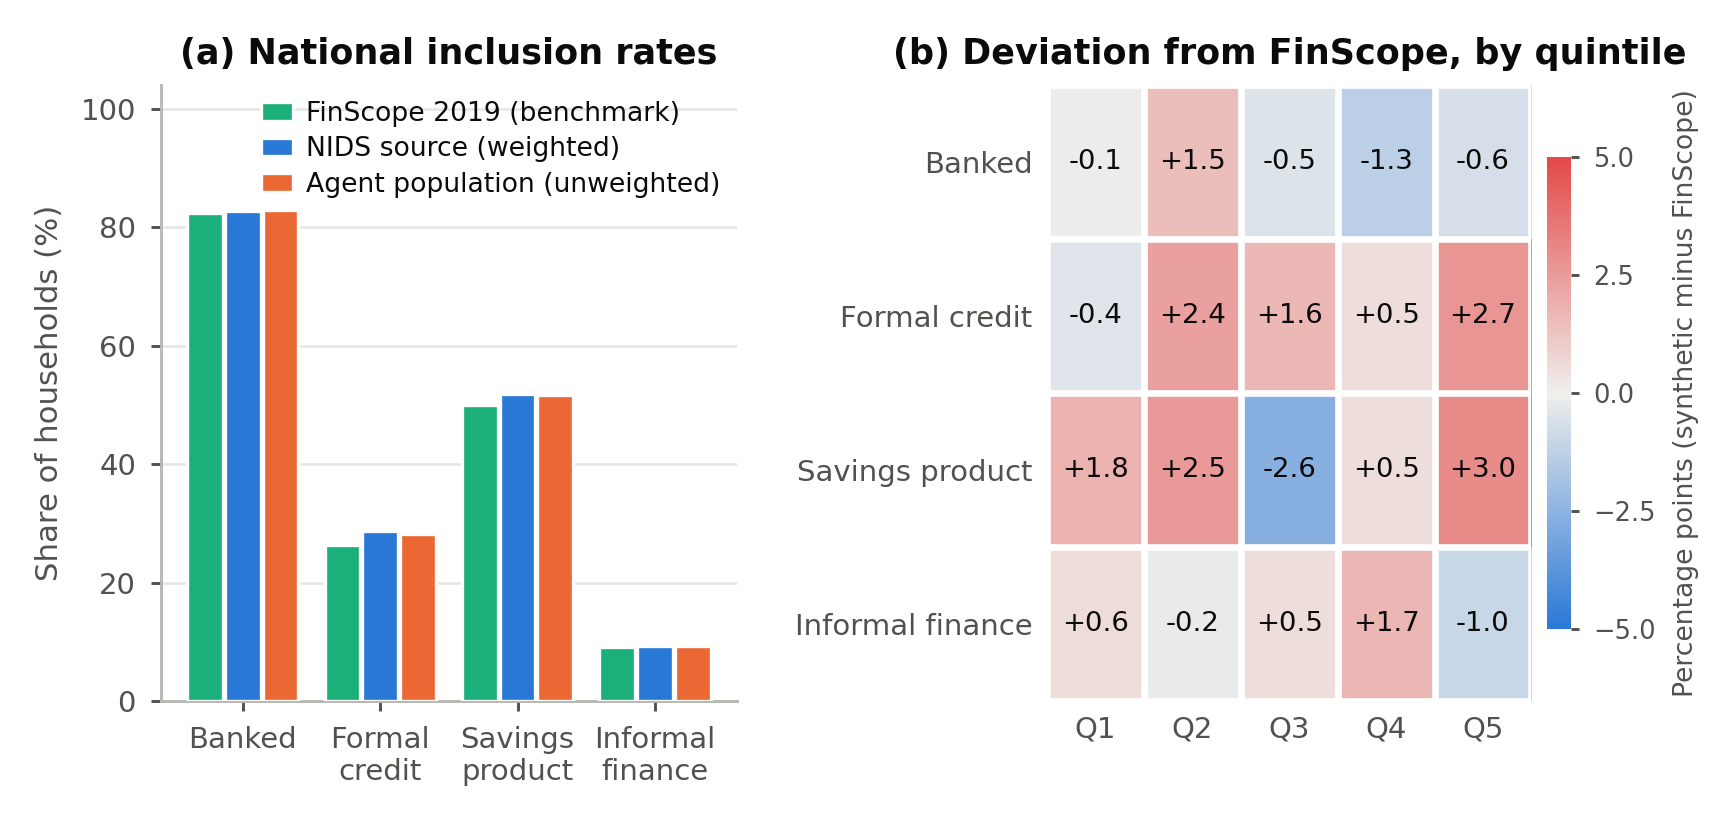
\includegraphics[width=\textwidth]{figures/fig_inclusion_fidelity.png}
\caption{Fidelity of the imputed indicators}
\label{fig:inclusion-fidelity}
\tabnote{Panel (a) compares the national rate of each of the six imputed indicators across the \ac{FinScope} 2019 target, the weighted synthetic population and the unweighted 5{,}000-agent population, as in Table~\ref{tab:imputation_errors}. Panel (b) shows the synthetic-less-\ac{FinScope} gap for each indicator within each per-capita income quintile, thirty cells in all; the largest single deviation is 2.3 percentage points against a tolerance of 5. Quintiles are the weighted \ac{NIDS} bounds of Appendix~\ref{app:variables}.}
\end{figure}

\begin{figure}[H]
\centering
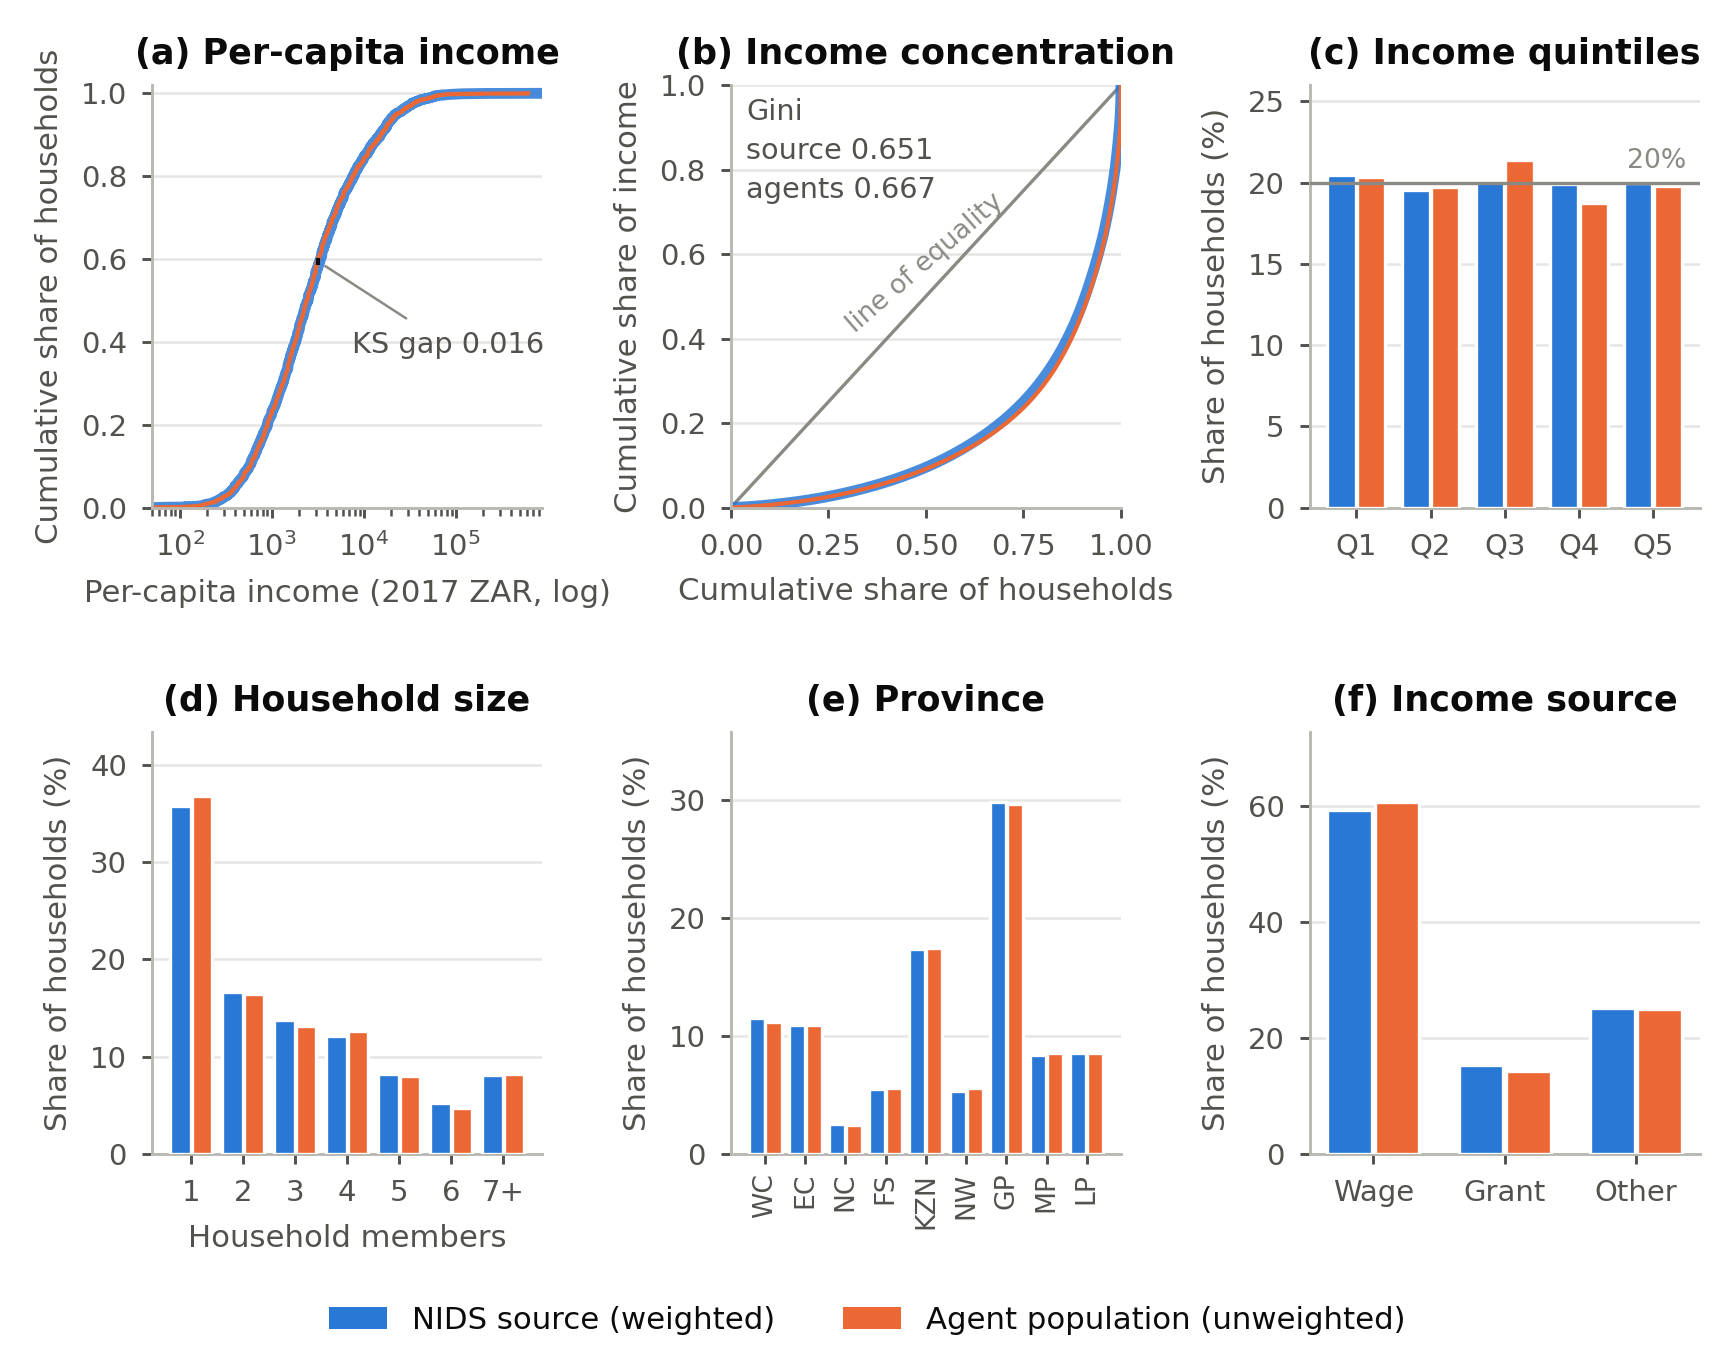
\includegraphics[width=\textwidth]{figures/fig_population_fidelity.png}
\caption{Distributional fidelity of the agent population}
\label{fig:pop-fidelity}
\tabnote{Each panel compares the unweighted 5{,}000-agent resample, drawn with replacement in proportion to \ac{NIDS} survey weight (seed 20260818) from 3{,}221 unique source records, against the weighted 10{,}841-household source it is drawn from. Panels (a) and (b) cover the per-capita income distribution and its concentration; panels (c) to (f) cover income quintile, household size, province and primary income source, the categorical attributes that gate behaviour and define the reference groups in the simulation. The Kolmogorov--Smirnov distance in (a) is 0.016, the largest categorical deviation across the 24 sub-categories is 1.4 percentage points, and the Gini rises by 0.015, from 0.6514 to 0.6668.}
\end{figure}
